\section{Mobilität}
  Durch die drei Campi in Heidelberg hat nicht jeder Student den Vorteil mitten
  in der Altstadt studieren zu können. Gerade die Naturwissenschaften mit ihren großen
  Laboren brauchten neuen Platz und mussten notgedrungen ``auswandern''. Unser Campus ist
  das Neuenheimer Feld und in sich auch sehr schön gestaltet.
  Aber grade abends und als Besucher will man doch gerne mal in die Stadt, also das
  ``originale'' Heidelberg.
  Als Einheimischer ist das Mittel der Wahl hier natürlich das Fahrrad, aber das wird wohl
  kaum einer von euch extra mitgenommen haben. Dazu haben wir euch ein paar Alternativen
  rausgesucht. Auf den letzten ZaPFen haben wir festgestellt, dass die Mobilitätstickets von den meisten
  nicht sehr häufig genutzt wurden. Darum haben wir in Heidelberg entschieden euch
  dieses Mal kein Ticket für das lange Wochenende zu organisieren.

  \subsection{öffentlicher Nahverkehr}
    Wer neben der Kneipentour hin und wieder gerne mal in die Altstadt möchte, der hatte bei
    der Anmeldung schon die Möglichkeit, sich eine HeidelbergCard zu kaufen.
    Es ist unsere günstige Empfehlung, um vor Ort stresfrei von A nach B zu kommen.
    Und ihr dürft sogar kostenfrei die Bergbahn auf den Königstuhl benutzen.
    Falls ihr euch doch spontan überlegt, abends mal die Bahnen zu nehmen, kann
    direkt in der Jugendherberge (Tiergartenstraße 5) ein Ticket für 19 \euro für die vier Tage
    erworben werden oder ihr holt euch eben je nach Bedarf Fahrscheine an den Automaten
    an den Bahnhaltestellen oder beim Fahrer.
    Das ist auch ganz praktisch, wenn ihr später am Abend mal zu faul seid, doch
    noch den ganzen Weg von den Kneipen zur Herberge zu laufen.
    Wahrscheinlich ist es für euch alle am schlausten, die HeidelbergCard erst
    Donnerstag zu kaufen damit ihr Sonntag nach dem Endplenum noch die Altstadt und
    den Königstuhl besuchen könnt, wenn ihr mit all den Plenen und
<<<<<<< HEAD
    AKs noch nicht genug zu tun habt. \\
    Streckenmäßig gibt es sogar zwei verschiedene Busse, die von der Jugendherberge
    bis in die Altstadt fahren. Die Linie \textbf{31} fährt von der Haltestelle
    \underline{Jugendherberge} über das \underline{Bunsengymnasium} bis zum
    \underline{Universitätsplatz} und wieder zurück mit der Zielhaltestelle
    \underline{Chirurgische Klinik}. Das Bunsengymnasium ist von den Arbeitsräumen
    die nächste Haltestelle. Stattdessen könnt ihr auch die Linie \textbf{32} nehmen,
    je nachdem welche grade passender ist. Sie fährt von der \underline{Jugendherberge}
    auch zum \underline{Universitätsplatz} und zurück bis zur \underline{Kopfklinik}.
    Jedoch könnt ihr dann nicht am \underline{Bunsengymnasium} ein- oder aussteigen.
        \todo{Busnetzplan Linien 31, 32}

=======
    AKs noch nicht genug zu tun habt.
>>>>>>> f55a69417578f628d9142c4b462f0efb0e5b69be
  \subsection{VRNnextbike}
    Der regionale Verkehrsverbund bietet auch Mietfahrräder an. Das ist eine super Gelegenheit
    für kleines Geld schnell in die Altstadt, den Bahnhof oder was auch immer zu kommen.
    Praktisch ist es besonders dann, wenn ihr am Start- und Zielort eine Verleihstation habt.
    Leider können wir euch hierfür kein Zeitticket anbieten, es gibt schlichtweg keins.
    Die Registrierung erfolgt allerdings kostenfrei und ist auf der folgenden Seite
    genauer beschrieben (\url{http://www.vrnnextbike.de/de/information/}).
    Für 1 \euro \, pro halber Stunde (maximal 9 \euro \, pro Ausleihe) gibt es ein verkehrstüchtiges
    Fahrrad und das sportliche Workout inklusive.
<<<<<<< HEAD
    % Gerade wenn ihr in der etwas abseits gelegenen Jugendherberge untergebracht seit,
    % macht das durchaus Sinn, da dort auch einige Räder direkt vor der Tür auf euch warten.
        \todo{VRNextbike direkt an der JH?}

    \begin{figure}
      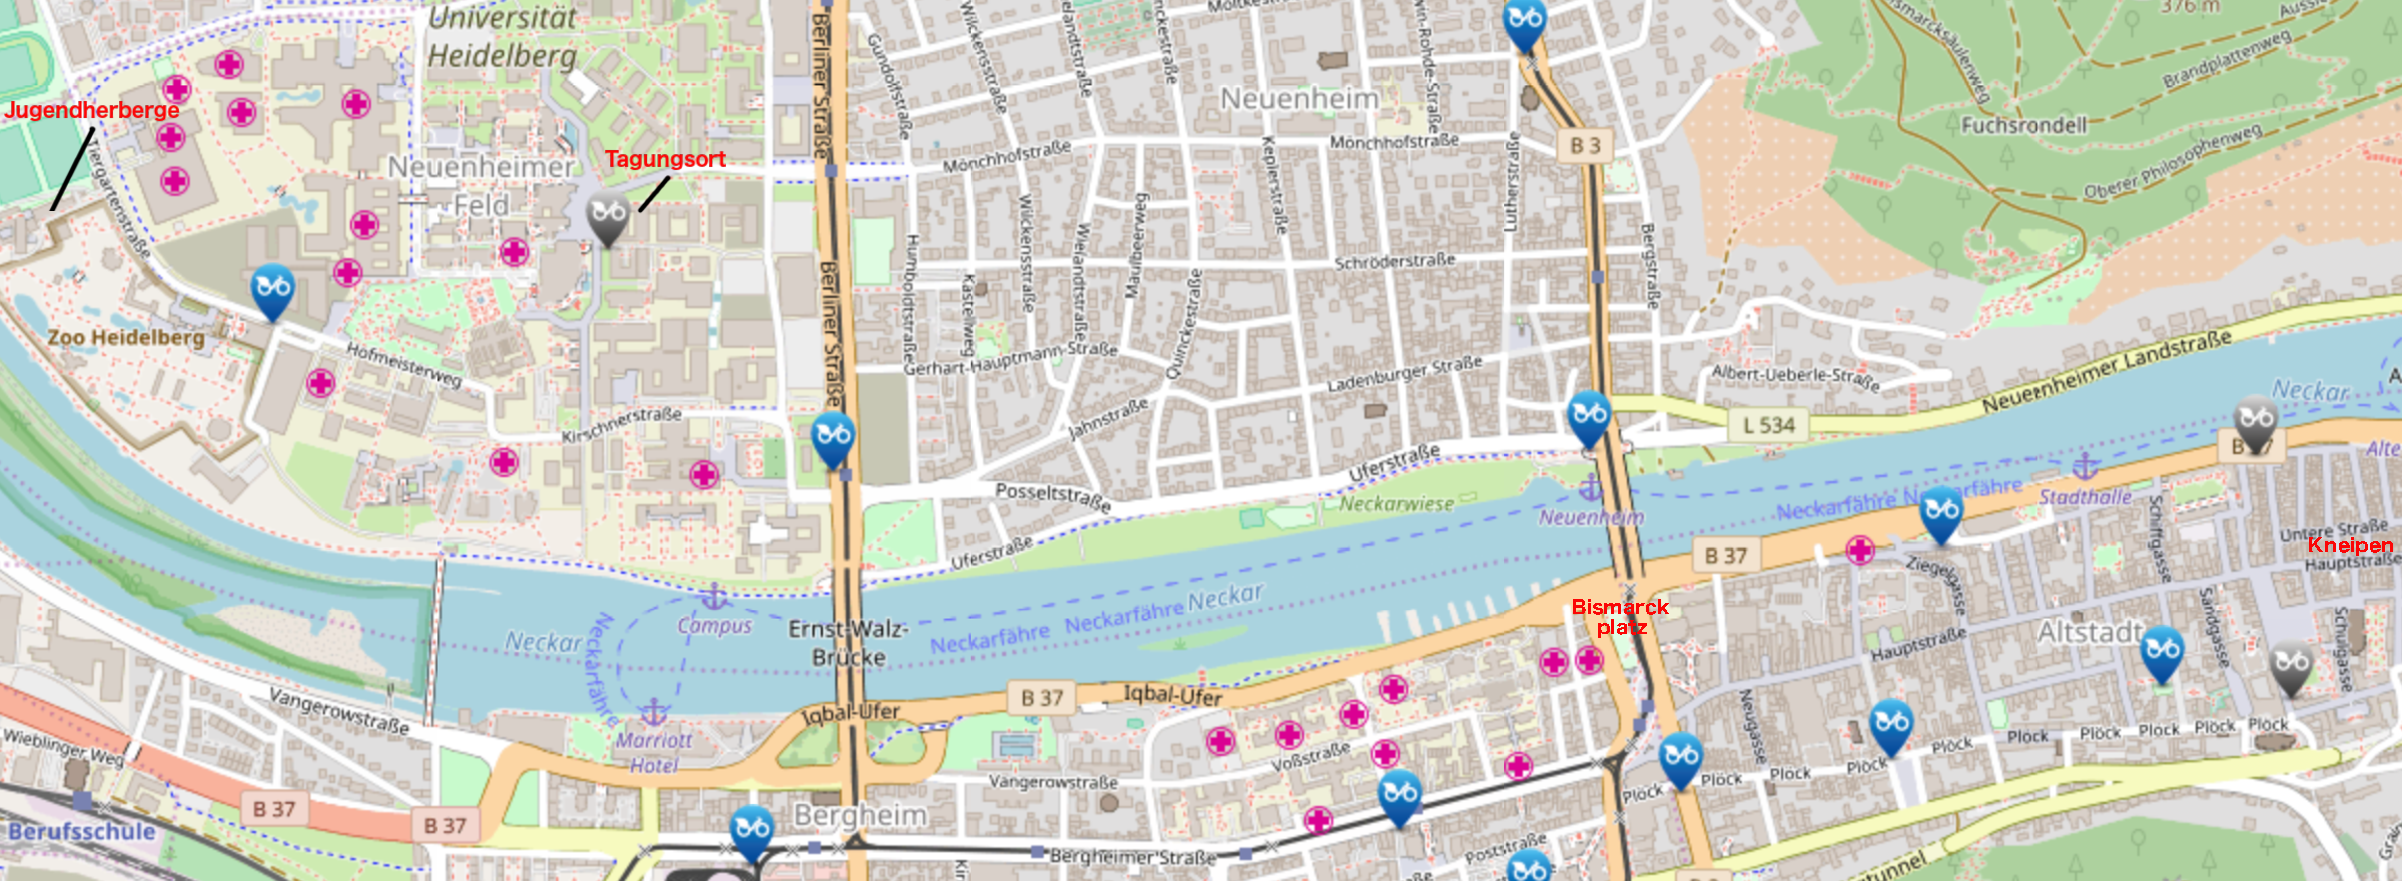
\includegraphics[width=1.0\textwidth]{chapters/mobilitaet/nextbike}
      \caption{Verlehistellen VRNnextbike}
      \label{nextbike}
    \end{figure}

=======
    Gerade wenn ihr in der etwas abseits gelegenen Jugendherberge untergebracht seit,
    macht das durchaus Sinn, da dort auch einige Räder direkt vor der Tür auf euch warten.
>>>>>>> f55a69417578f628d9142c4b462f0efb0e5b69be
    Und nicht zuletzt ist Heidelberg eine sehr Radfahrer freundliche Stadt.
